\documentclass[conference]{IEEEtran}
\IEEEoverridecommandlockouts
% The preceding line is only needed to identify funding in the first footnote. If that is unneeded, please comment it out.
\usepackage{cite}
\usepackage{amsmath,amssymb,amsfonts}
\usepackage{algorithmic}
\usepackage{graphicx}
\usepackage{textcomp}
\usepackage{xcolor}
\usepackage{float}
\usepackage{array}


\def\BibTeX{{\rm B\kern-.05em{\sc i\kern-.025em b}\kern-.08em
    T\kern-.1667em\lower.7ex\hbox{E}\kern-.125emX}}
\begin{document}

\title{Assignment 1: Supervised Learning\\
}

\author{\IEEEauthorblockN{[Jainil Modi]}
\IEEEauthorblockA{\textit{[jmodi30@gatech.edu]}}
}

\maketitle

\section{Introduction - Dataset Explanation}

\subsection{Preface and Acknowledgements}
For this project, I used a mixture of my own code and ChatGPT for help with explanation. Specifically, because I know my datasets are canonical, ChatGPT was really helpful in describing the attributes, as well as helping me interpret my graphs (for example, I asked it how to interpret a validation curve). 

\subsection{Dataset 1: PIMA Indians Diabetes Dataset}
The first dataset I have is regarding the presence (or lack thereof) of diabetes. There are 9 attributes, including the target attribute. They are as follows: Pregnancies: no. of times pregnant, Glucose: Plasma glucose concentration after a 2-hour oral glucose tolerance test, BloodPressure: Diastolic BP (mm Hg), SkinThickness: Triceps skinfold thickness (mm), Insulin: 2-Hour serum insulin (mu U/ml), BMI: (weight in kg / (height in m)\^2), DiabetesPedigreeFunction: a measure of the diabetes genetic influence, and Age. 

\subsection{Dataset 2: Red Wine Quality}
The second dataset I have is regarding wine quality. There are 13 attributes, including the target attribute, which is of course the quality of the wine. They are as follows: ID, fixedacidity: the concentration of non-volatile acids (grams/liter), volatileacidity: (grams/liter), citricacid: (grams/liter), residualsugar: (grams/liter), chlorides: salt concentration (grams/liter), freesulfurdioxide: parts per million, or ppm, totalsulfurdioxide: expressed in ppm, density: g/mL, pH: unitless, sulphates: grams of potassium sulphate/liter, alcohol: percentage of alcohol by volume of wine, quality: ranging from 3 to 8. Higher values indicate better quality. 

\subsection{Preprocessing and Hyperparameter of Focus}
For both datasets, I chose to use the f1\_weighted metric: When the outcome variables for both datasets are not uniform or normally distributed, f1\_weighted score helps even things out.


\begin{figure}[H]
    \centering
    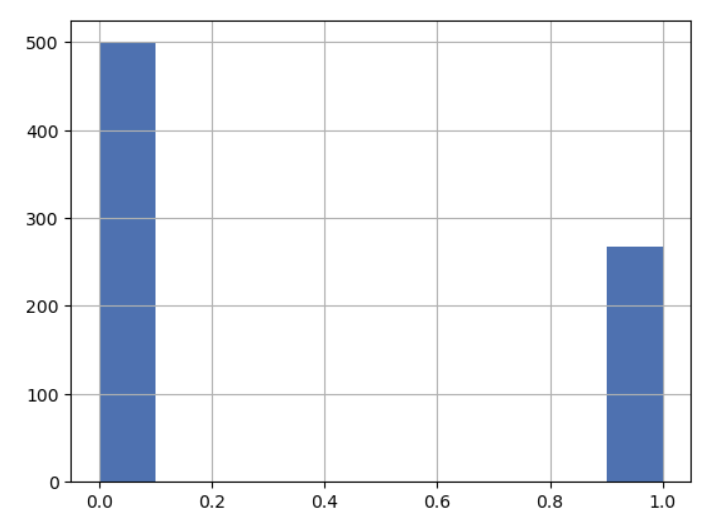
\includegraphics[width=0.40\textwidth]{Preprocessing Graphs/pima outcome var.png}
    \label{fig:enter-label}
    \caption{Presence of Diabetes labeled as 1, else 0}
\end{figure}

 \begin{figure}[H]
    \centering
    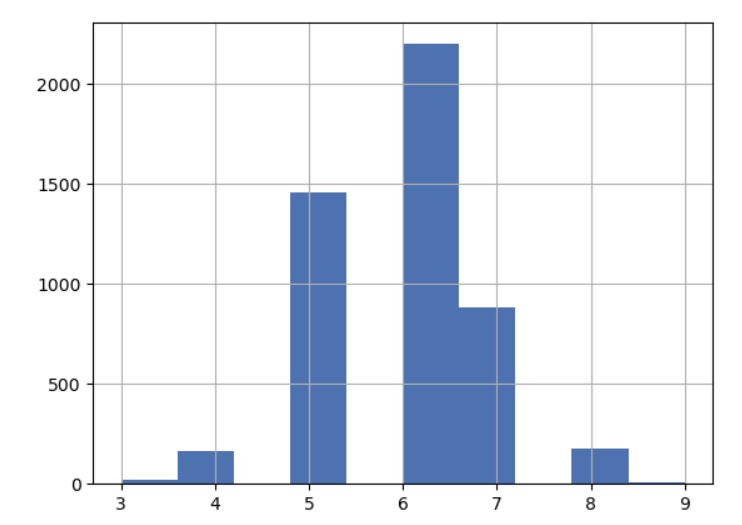
\includegraphics[width=0.40\textwidth]{Preprocessing Graphs/rwq outcome var.png}
    \label{fig:enter-label}
    \caption{Distribution of Wine Quality}
\end{figure}


\section{Decision Trees}

\subsection{\textbf{PIMA Indians Diabetes Dataset}}\label{AA}
For this dataset, the goal is predict the presence of diabetes, and therefore, the problem is one of classification. The ccp\_alpha score I chose to initialize with was 0.005. With this, my baseline MAE value was 0.18796, which is poor. After hyperparameterization using GridSearchCV, it increased to 0.745041. 

\begin{figure}[H]
    \centering
    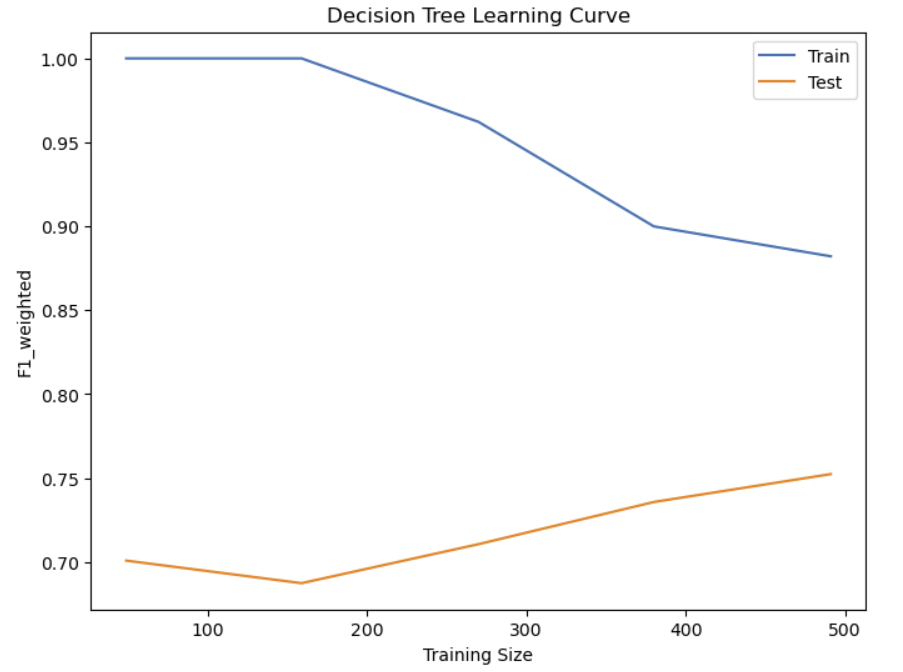
\includegraphics[width=0.40\textwidth]{PIMA Indian Diabetes Graphs/Decision Trees/dt pima init.png}
    \label{fig:enter-label}
    \caption{Initial Decision Tree Learning Curve}
\end{figure}

\begin{figure}[H]
    \centering
    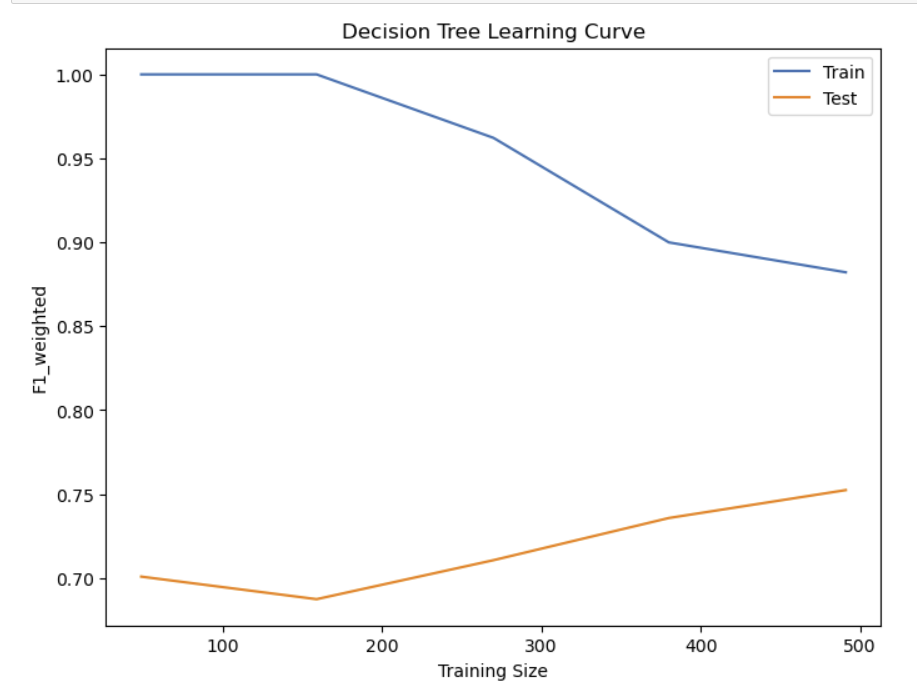
\includegraphics[width=0.40\textwidth]{PIMA Indian Diabetes Graphs/Decision Trees/dt pima final.png}
    \label{fig:enter-label}
    \caption{Final Decision Tree Learning Curve}
\end{figure}
    
As seen from the graphs, it is evident that there is high variance in this particular dataset. The dataset seems to converge later on with more and more examples. Even after hyperparameterization, this learning curve does not improve much. With the validation curve, I chose to plot f1\_weighted versus ccp\_alpha. It was interesting to see that after 0.005, the f1\_weighted score levels off around 0.005. This means that the decision tree will not prune more nodes off. After attempting to prune the tree, the initial ccp\_alpha value happened to be the best. 

\begin{figure}[H]
    \centering
    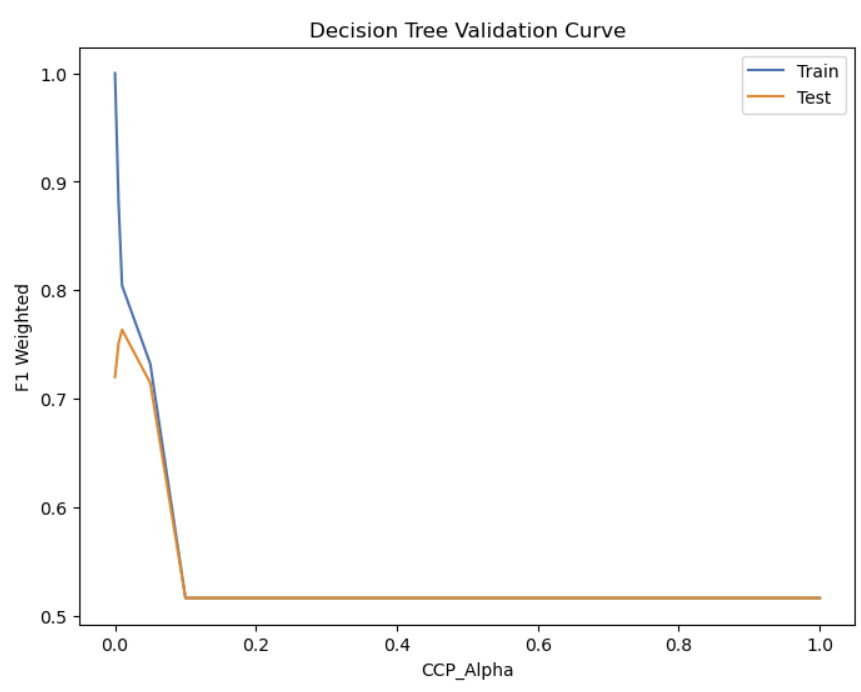
\includegraphics[width=0.40\textwidth]{PIMA Indian Diabetes Graphs/Decision Trees/dt val curve.png}
    \label{fig:enter-label}
\end{figure}

As for wall clock time, training and testing were relatively quick. Fitting the data took a third of the time that it did to train the dataset. See below for wall clock time:

\begin{figure}[H]
    \centering
    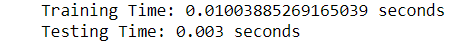
\includegraphics[width=0.40\textwidth]{PIMA Indian Diabetes Graphs/Decision Trees/dt wct.png}
    \label{fig:enter-label}
\end{figure}

Overall, the decision tree did a fair job at classifying the data. This is evidenced by a high precision and high recall score. See the classification report below: 

\begin{figure}[H]
    \centering
    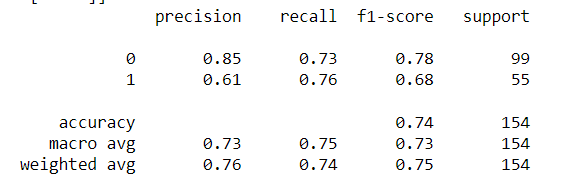
\includegraphics[width=0.40\textwidth]{PIMA Indian Diabetes Graphs/Decision Trees/dtcr.png}
    \label{fig:enter-label}
\end{figure}
    
The precision score was great, and that was likely due to the imbalance of 0s. Recall could have been better, as it performs just slightly better than chance. F1-score weighted performed well: being on a scale of 0 to 1, where 1 is better, a 0.75 score indicates that this algorithm was able to learn fairly well. 

\subsection{\textbf{Red Wine Quality}}\label{BB}
For this dataset, I started with a ccp\_alpha of 0.005. With this initial tree, I get an f1\_weighted score of about 0.4605. 

\begin{figure}[H]
    \centering
    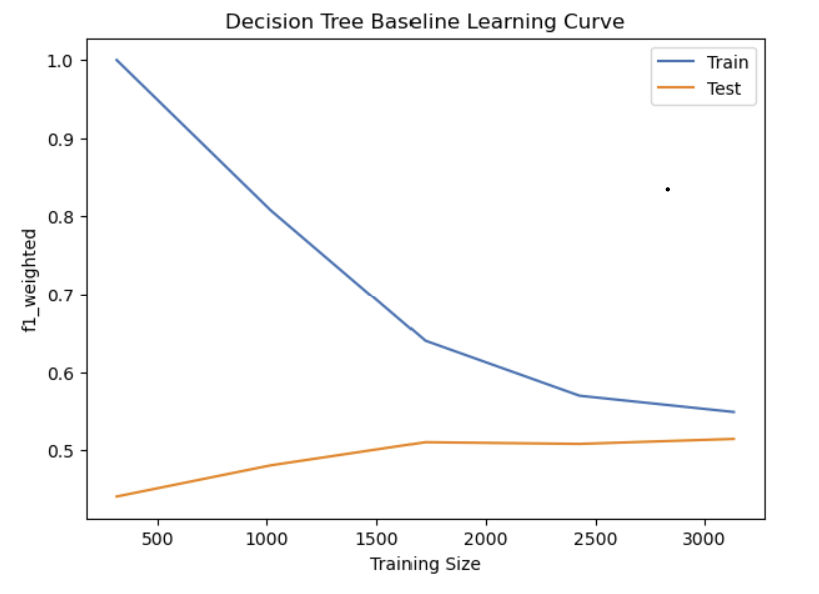
\includegraphics[width=0.40\textwidth]{Red Wine Quality Graph Images/Decision Trees/dt lc init.png}
    \label{fig:enter-label}
\end{figure}

After looking at this graph, there is a lot of variance in the dataset, but not so much bias. What I take away from this is that the algorithm that I started with is overfitting. A model that has low bias and high variance tends to overfit. In order to find parameters that better suit the data, I used GridSearchCV for hyperparameterization. From there, I used the suggested 0 for ccp\_alpha, entropy for 'criterion', and a max\_depth of 20. I think it is interesting that this dataset and particular algorithm actually benefit from little-to-no pruning. Additionally, I included the wall clock time as a table, to illustrate how quickly the training and testing sets are fit to decision tree. See below for the updated learning curve, validation curve, and the wall clock time.

\begin{figure}[H]
    \centering
    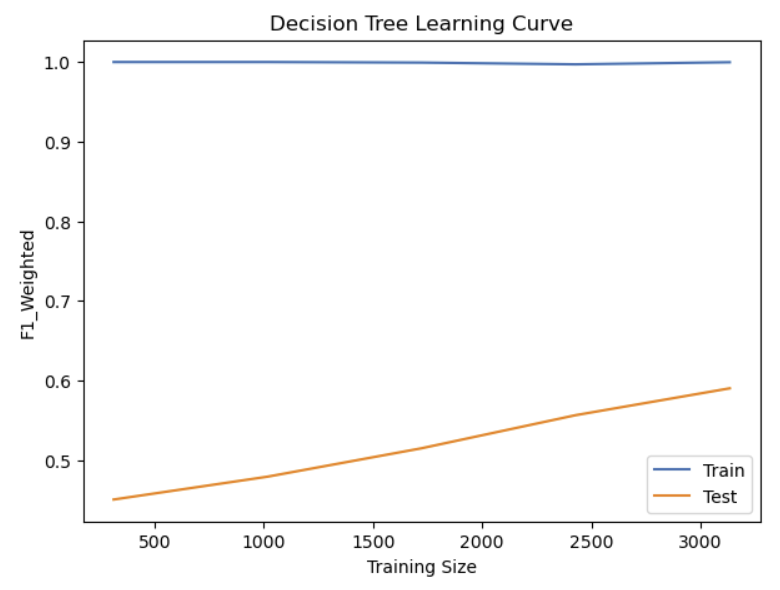
\includegraphics[width=0.40\textwidth]{Red Wine Quality Graph Images/Decision Trees/dt lc final.png}
    \label{fig:enter-label}
\end{figure}

\begin{figure}[H]
    \centering
    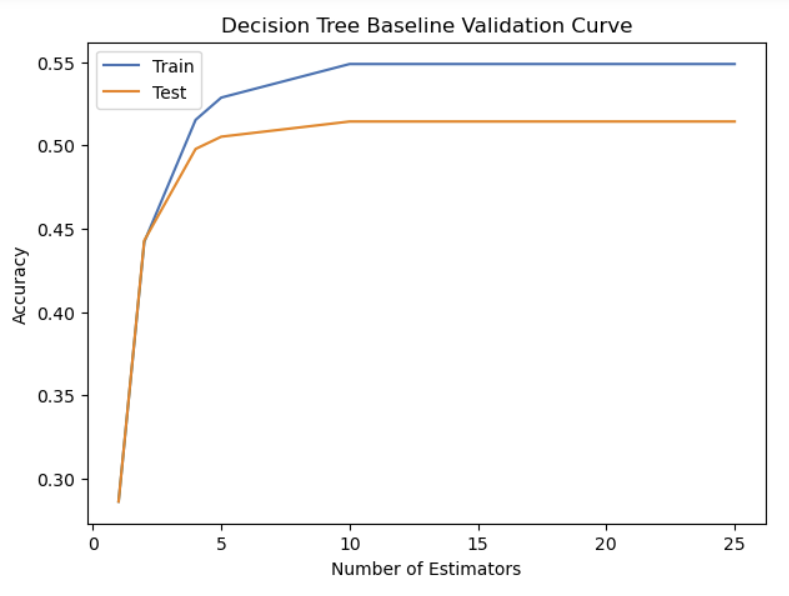
\includegraphics[width=0.40\textwidth]{Red Wine Quality Graph Images/Decision Trees/dtc valid curve.png}
    \label{fig:enter-label}
\end{figure}

\begin{figure}[H]
    \centering
    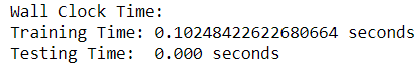
\includegraphics[width=0.40\textwidth]{Red Wine Quality Graph Images/Decision Trees/dtc wall clock time.png}
    \label{fig:enter-label}
\end{figure}

From the image above, it is demonstrable that once the algorithm is tuned, the data fit almost instantaneously. I went to three digits after the decimal to the test fit time, and they were still all zeros.

\begin{figure}[H]
    \centering
    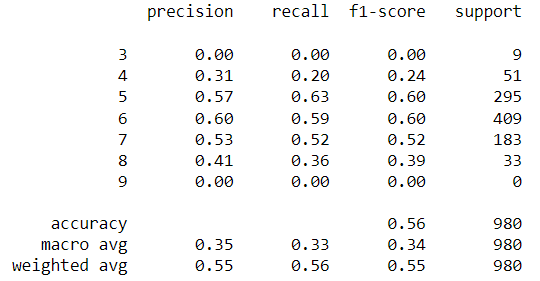
\includegraphics[width=0.40\textwidth]{Red Wine Quality Graph Images/Decision Trees/dtc cm.png}
    \label{fig:enter-label}
\end{figure}

The table above shows that the resulting f1-score 0.55, a 0.9 increase from the initial tree. It even got 5s right over 50\% of the time, and 4s about one-third of the time. 

\section{KNN}

\subsection{\textbf{PIMA Indians Diabetes Dataset}}\label{AA}
When compared to the other sections, this dataset trains very quickly. The starting tree was made out with 10 neighbors. This already gave me a 0.6794 f1\_weighted score. Not so surprisingly, the final f1\_weighted score slightly improved: 0.71537. 

\begin{figure}[H]
    \centering
    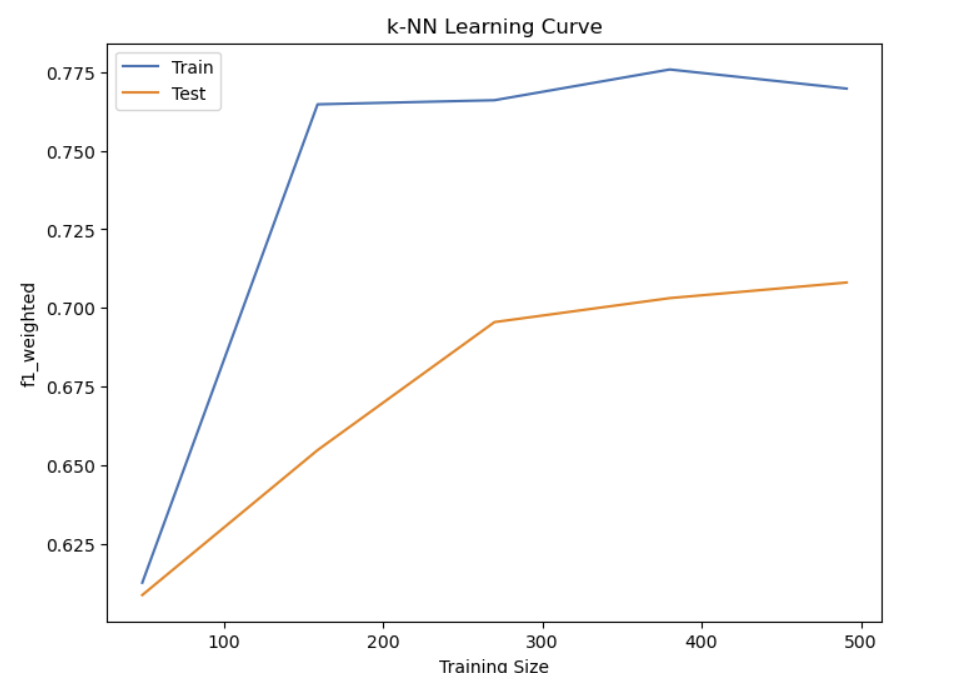
\includegraphics[width=0.40\textwidth]{PIMA Indian Diabetes Graphs/KNN/knn init lc.png}
    \label{fig:enter-label}
\end{figure}

This representation of the data illustrates a picture the is little variance, but high bias in the distribution. The curves do not seem to want to converge a singular value, in fact, quite the opposite. 
This demonstrates that the KNN model is underfitting the given data.

From the testing plot, it became evident that the GridSearchCV model was overfitting: 

\begin{figure}[H]
    \centering
    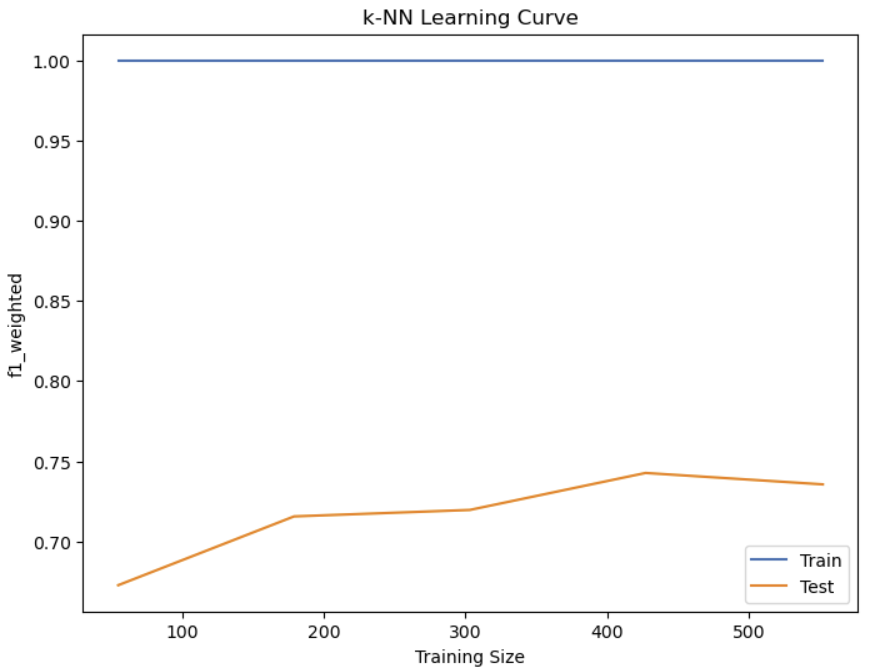
\includegraphics[width=0.40\textwidth]{PIMA Indian Diabetes Graphs/KNN/knn fin lc.png}
    \label{fig:enter-label}
    \caption{Training curve has a perfect f1\_weighted score, but test curve does not, and seems to taper around 0.75.}
\end{figure}

One possible reason for this perfect score is the fact that the initial algorithm already started with the best number of neighbors. Additionally, because the 'algorithm' parameter is defaulted to 'auto', it finds the best option as is. Lastly, the GridSearchCV also changed the weights of each neighbor from 'uniform' to 'distance', which gives points that are closer to a query point more influence. 

From the validation curve below, it is evident that after 10 neighbors, the algorithm does not benefit very much, if at all: 

\begin{figure}[H]
    \centering
    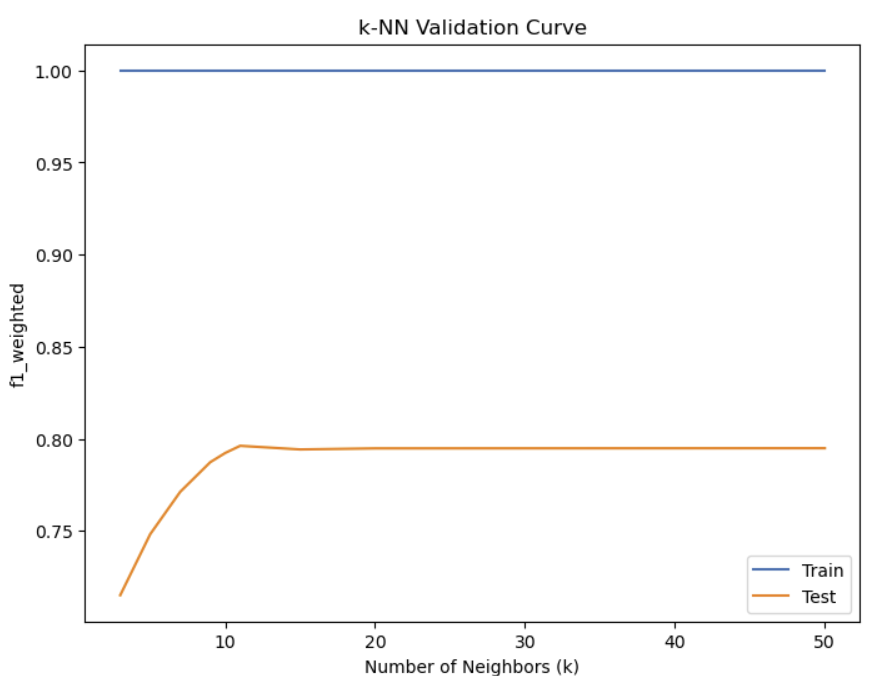
\includegraphics[width=0.40\textwidth]{PIMA Indian Diabetes Graphs/KNN/knn vc.png}
    \label{fig:enter-label}
    \caption{After 10 neighbors, the f1\_weighted score remains stagnant.}
\end{figure}

The one thing that KNN had on its 'peers' was the training time and test time. Per pair, it was computed the fastest. 

\begin{figure}[H]
    \centering
    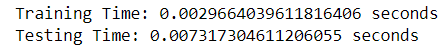
\includegraphics[width=0.40\textwidth]{PIMA Indian Diabetes Graphs/KNN/knn wct.png}
    \label{fig:enter-label}
    \caption{Training time was the fastest of all algorithms for this dataset.}
\end{figure}

\subsection{\textbf{Red Wine Quality}}\label{BB}

The initial K value I chose for this dataset was the default, which is 5. From this, the f1\_weighted score was 0.528472, so a better start than the Adaboost implementation with this dataset. 

\begin{figure}[H]
    \centering
    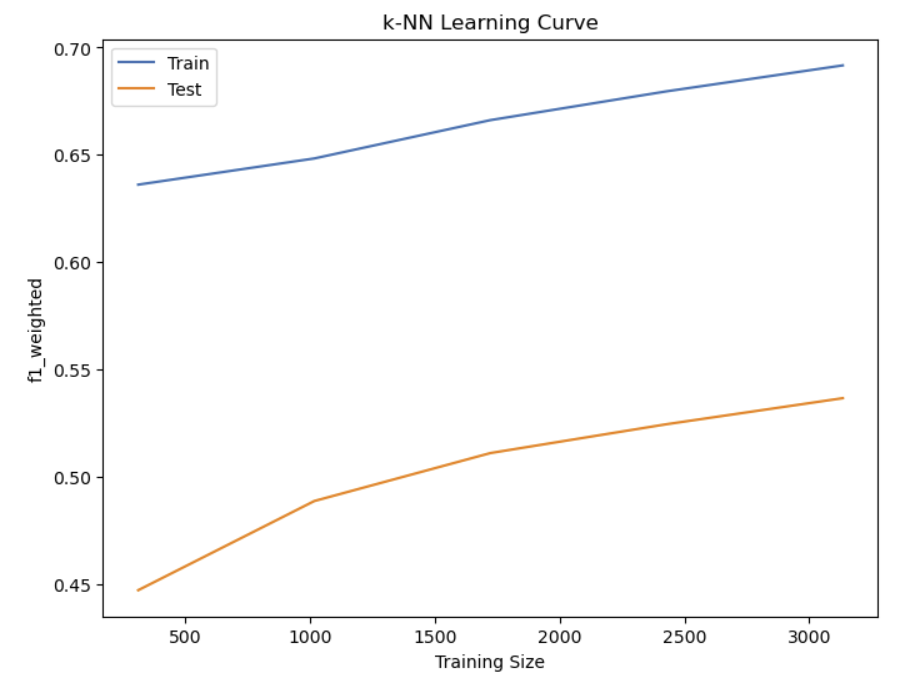
\includegraphics[width=0.40\textwidth]{Red Wine Quality Graph Images/KNN/knn lc init.png}
    \label{fig:enter-label}
    \caption{High variance and high bias in initial stages.}
\end{figure}

\begin{figure}[H]
    \centering
    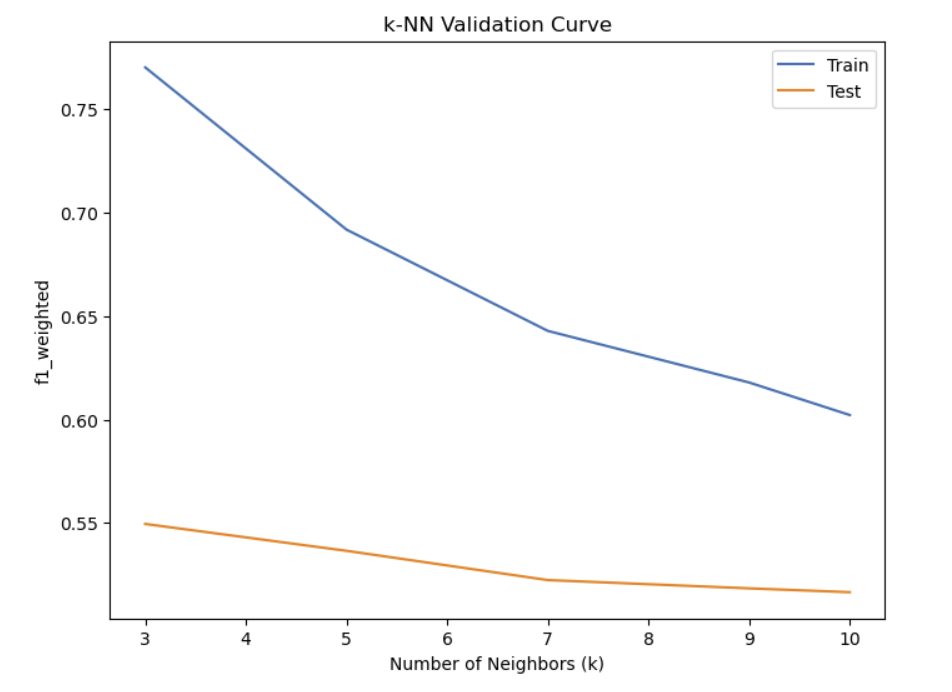
\includegraphics[width=0.40\textwidth]{Red Wine Quality Graph Images/KNN/knn vc init.png}
    \label{fig:enter-label}
    \caption{F1\_weighted score performs objectively worse with an increase in the number of neighbors (k)}
\end{figure}

After consulting GridSearchCV, the following hyperparameters were deemed optimal: algorithm='ball\_tree', n\_neighbors=50, weights='distance'. Similar to the PIMA Indians Diabetes dataset, the algorithm chose both ball\_tree for the algorithm and distance for the weights. 

\begin{figure}[H]
    \centering
    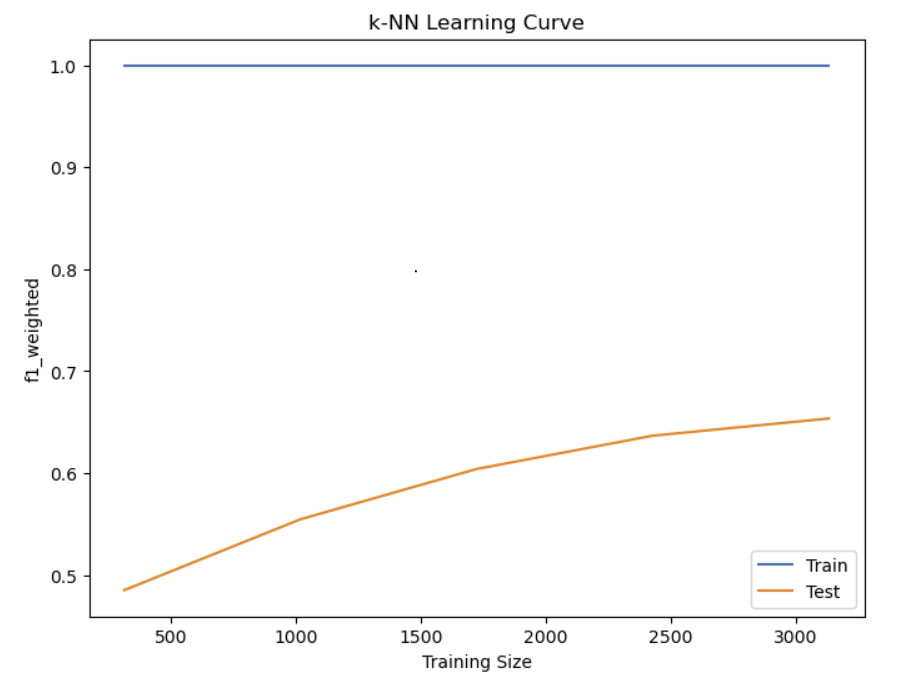
\includegraphics[width=0.40\textwidth]{Red Wine Quality Graph Images/KNN/knn lc final.png}
    \label{fig:enter-label}
    \caption{}
\end{figure}
\begin{figure}[H]
    \centering
    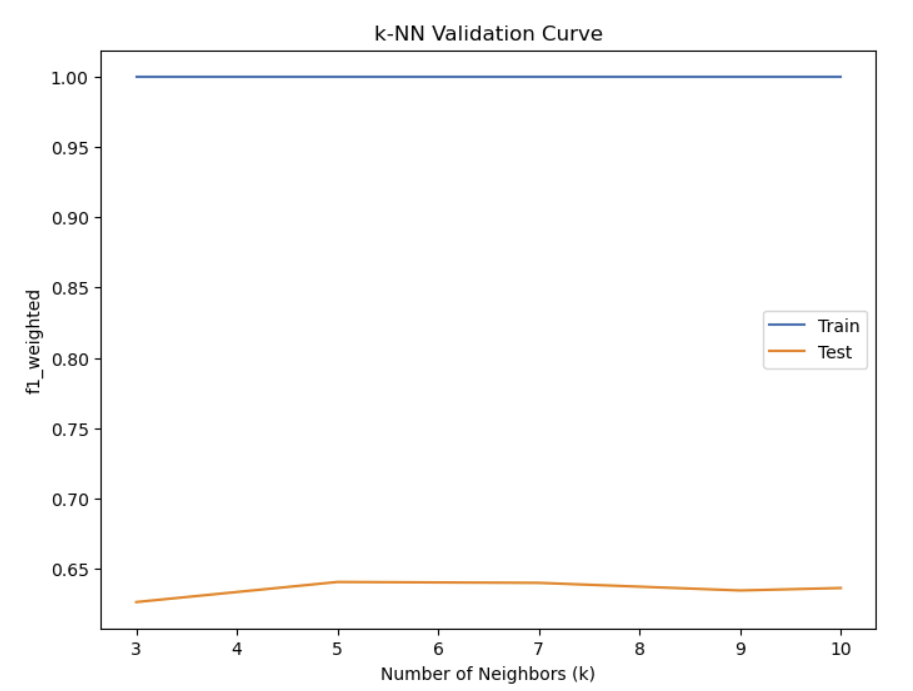
\includegraphics[width=0.40\textwidth]{Red Wine Quality Graph Images/KNN/knn vc final.png}
    \label{fig:enter-label}
    \caption{}
\end{figure}

\begin{figure}[H]
    \centering
    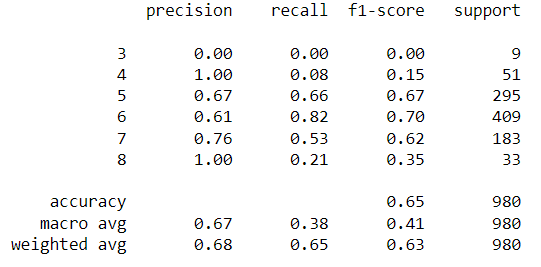
\includegraphics[width=0.40\textwidth]{Red Wine Quality Graph Images/KNN/knn cr.png}
    \label{fig:enter-label}
    \caption{Precision for both 4s and 8s much better here than anywhere else}
\end{figure}
\begin{figure}[H]
    \centering
    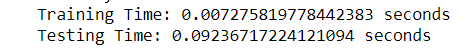
\includegraphics[width=0.40\textwidth]{Red Wine Quality Graph Images/KNN/knn wct.png}
    \label{fig:enter-label}
    \caption{Training time one of, if not, the fastest.}
\end{figure}

\section{Boosting}
For this ensemble method, I chose to use AdaBoosting. 

\subsection{\textbf{PIMA Indians Diabetes Dataset}}\label{AA}
I was anticipating the best f1\_weighted scores to come from this section. The reason is that in lecture material, we discussed how boosting cannot {\emph{really}} overfit. Because of it the inherent nature of this learning algorithm, I think the baseline performed really well: the initial f1\_weighted was 0.65517, much better than the decision tree's initial f1\_weighted score, for example. 

\begin{figure}[H]
    \centering
    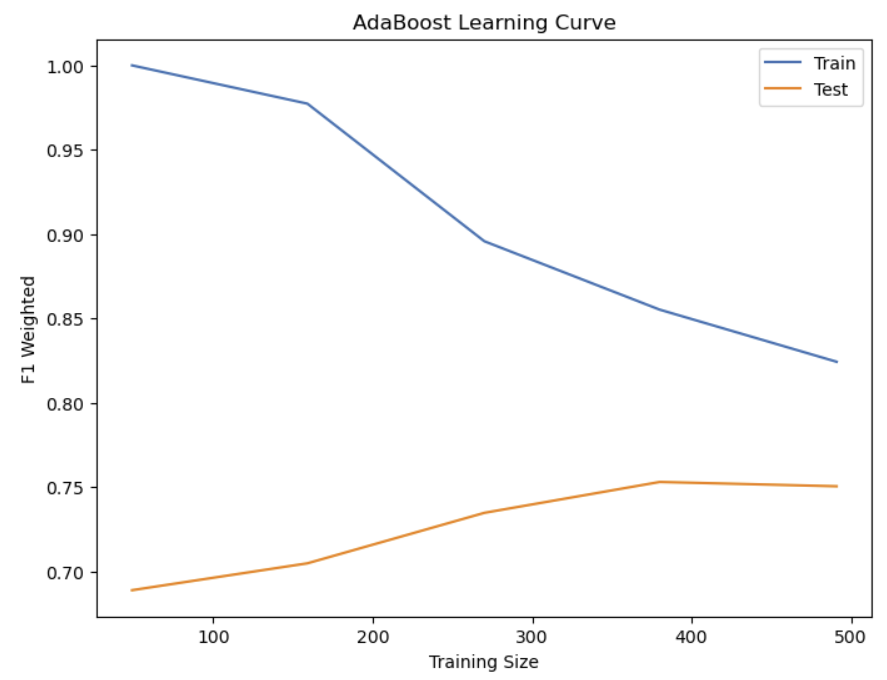
\includegraphics[width=0.40\textwidth]{PIMA Indian Diabetes Graphs/Adaboost/ada init lc.png}
    \label{fig:enter-label}
    \caption{There is high variance in the data, but it seems to converge later. There is still a presence of bias, however.}
\end{figure}

I initialized the adaboost with a decision tree classifier that had a max\_depth of 1, and a ccp\_alpha of 0.005. A very shallow tree, as is the requirement of an algorithm like this. For the adaboost, I initialized {\emph{its}} parameters with the base classifier, and n\_estimators=50, and a random\_state of 42 for reproducibility. After using GridSearchCV on the following parameters: n\_estimators, learning\_rate, and algorithm, this updated algorithm produce an f1\_weighted score of 0.742918. I think this is due to the algorithm choosing SAMME.R, and going off of the probability, because there are not many records to reference. 

\begin{figure}[H]
    \centering
    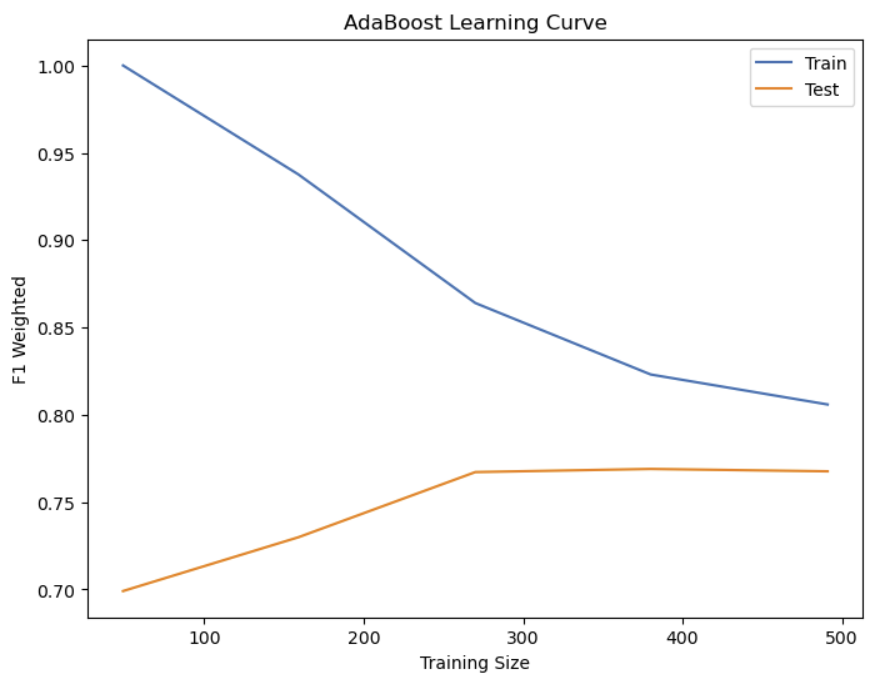
\includegraphics[width=0.40\textwidth]{PIMA Indian Diabetes Graphs/Adaboost/ada fin lc.png}
    \label{fig:enter-label}
    \caption{Similar to the original curve with high variance, but a much smaller gap at the end, illustrating a larger potential for converging to a value.}
\end{figure}

This validation curve was the strangest one of the five for this dataset. It seems to suggest that the training set performs much better with a relatively small change in number of estimators, whereas it suggests that the test set will not grow as effectively, and it caps off quicker as well. 

\begin{figure}[H]
    \centering
    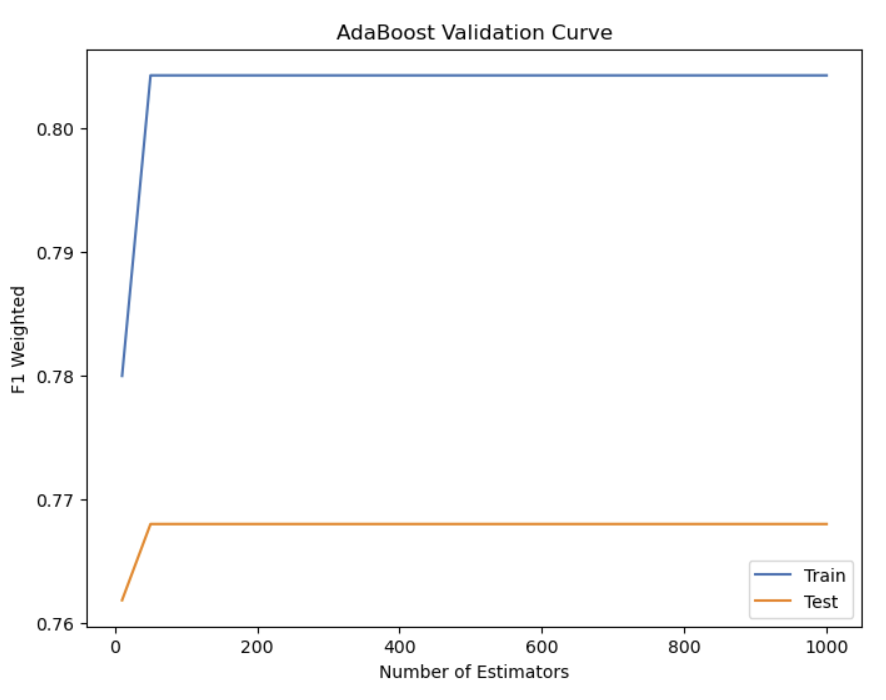
\includegraphics[width=0.40\textwidth]{PIMA Indian Diabetes Graphs/Adaboost/ada vc.png}
    \label{fig:enter-label}
    \caption{As mentioned above, a higher number of estimators does not result in much gain of f1\_weighted score for the validation set.}
\end{figure}

The adaboost algorithm perform exceptionally well for precision, but only got recall correct about two-thirds of the time. Below you can see the classification report: 

\begin{figure}[H]
    \centering
    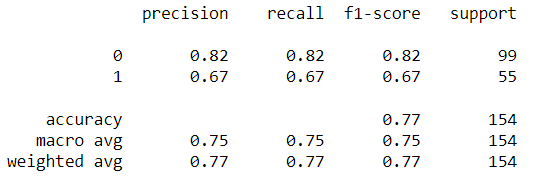
\includegraphics[width=0.40\textwidth]{PIMA Indian Diabetes Graphs/Adaboost/ada cr.png}
    \label{fig:enter-label}
    \caption{f1\_weighted score does well at 0.77}
\end{figure}

Wall Clock Time:
\begin{figure}[H]
    \centering
    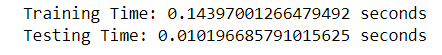
\includegraphics[width=0.40\textwidth]{PIMA Indian Diabetes Graphs/Adaboost/ada wct.png}
    \label{fig:enter-label}
    \caption{Training time was \emph{significantly} greater than testing}
\end{figure}

\subsection{\textbf{Red Wine Quality Dataset}}\label{BB}
My anticipation and results were way off for this algorithm and dataset combination. My baseline f1\_weighted score was 0.3590, which is to be expected, as it is supposed to take a weak learner. However, even after an extensive search with GridSearchCV to find the best hyperparameter combination, the score only improved to 0.44258. 

\begin{figure}[H]
    \centering
    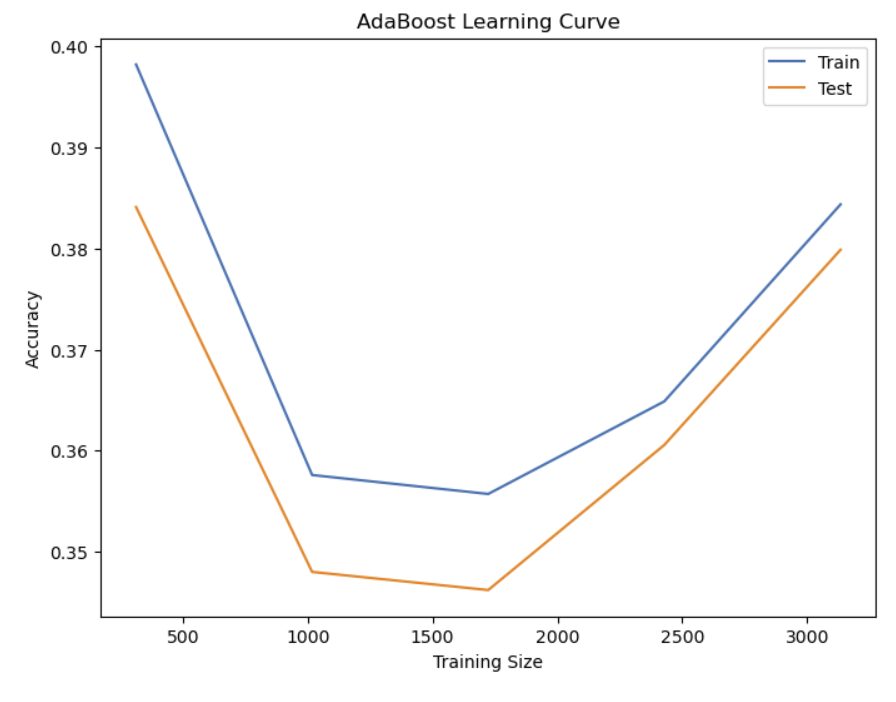
\includegraphics[width=0.40\textwidth]{Red Wine Quality Graph Images/Adaboost/ada lc init.png}
    \label{fig:enter-label}
    \caption{The training and test set benefit for lots of data, particularly after roughly 1750 records.}
\end{figure}

\begin{figure}[H]
    \centering
    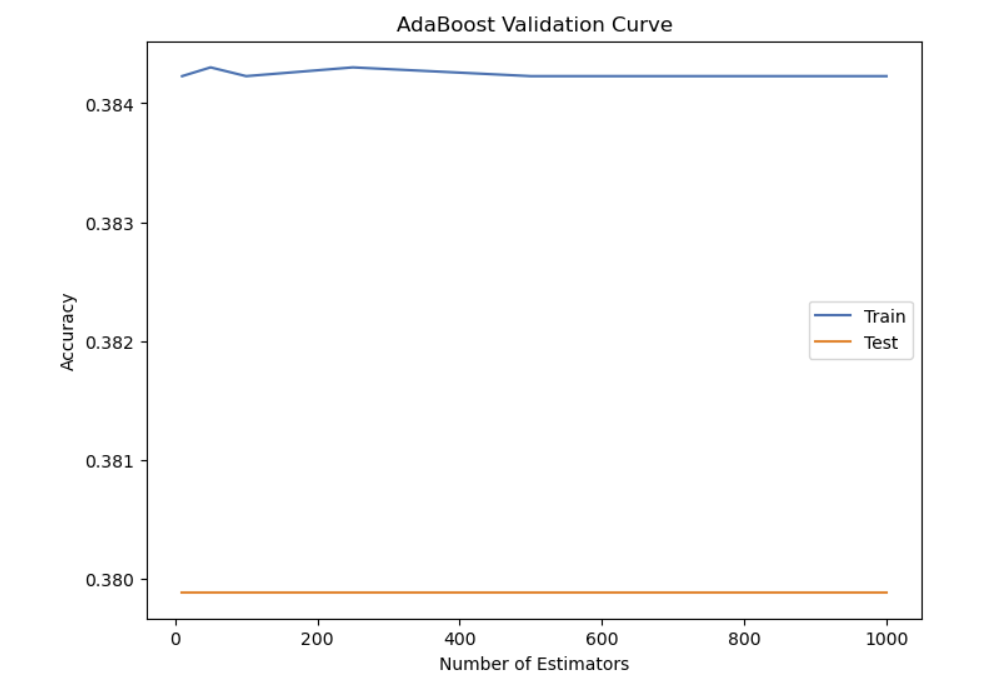
\includegraphics[width=0.40\textwidth]{Red Wine Quality Graph Images/Adaboost/ada vc init.png}
    \label{fig:enter-label}
    \caption{The f1\_score does not improve for either training nor testing}
\end{figure}

\begin{figure}[H]
    \centering
    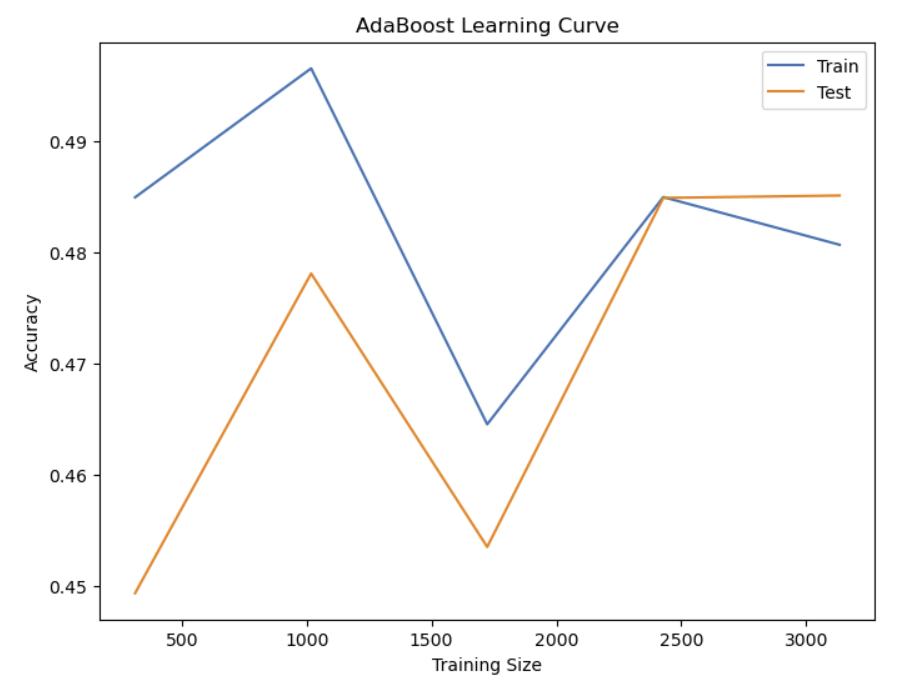
\includegraphics[width=0.40\textwidth]{Red Wine Quality Graph Images/Adaboost/ada lc final.png}
    \label{fig:enter-label}
    \caption{The more data they see, the worse they actually performed. At about 2500 records, both f1\_weighted scores begin to stagnate}
\end{figure}

\begin{figure}[H]
    \centering
    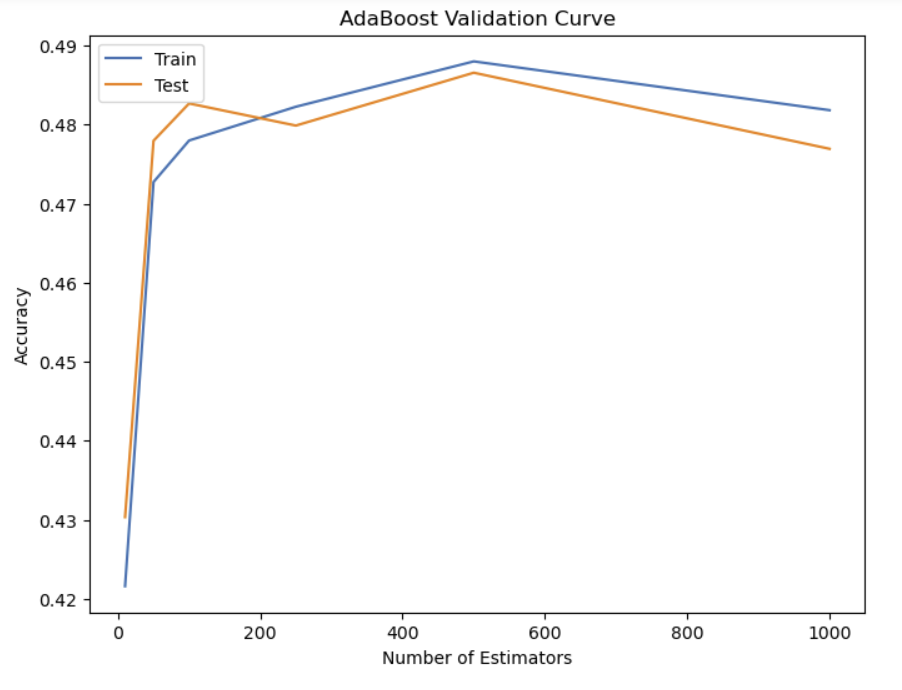
\includegraphics[width=0.40\textwidth]{Red Wine Quality Graph Images/Adaboost/ada vc final.png}
    \label{fig:enter-label}
    \caption{Both training and test sets peak at about the same number of estimators, that being around 500, but neither are doing particularly well, with an f1\_weighted score of ~0.485.}
\end{figure}

As indicated by the poor f1\_weighted score, the classification report was not good. 

\begin{figure}[H]
    \centering
    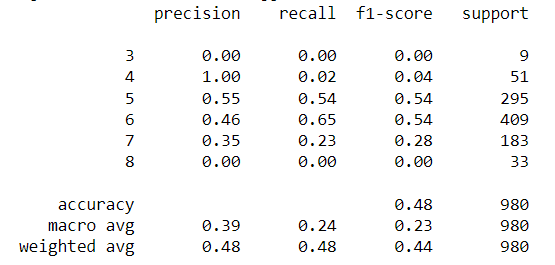
\includegraphics[width=0.40\textwidth]{Red Wine Quality Graph Images/Adaboost/ada cr.png}
    \label{fig:enter-label}
    \caption{Did poorly on all of the labels of quality.}
\end{figure}

\begin{figure}[H]
    \centering
    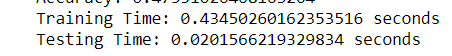
\includegraphics[width=0.40\textwidth]{Red Wine Quality Graph Images/Adaboost/ada wct.png}
    \label{fig:enter-label}
    \caption{Not as slow as SVMs on training.}
\end{figure}


\section{Neural Networks}
For this section, I choose to use the Multi-Layered Perceptron (MLP). 

\subsection{\textbf{PIMA Indians Diabetes Dataset}}\label{AA}
For my baseline MLP, I initialized it with the following parameters: {max\_iter=1000}, {early\_stopping=True}, {validation\_fraction=0.1}, {n\_iter\_no\_change=10},  {random\_state=42}, and {learning\_rate\_init=0.001}. From this, my initial f1\_weighted score was 0.51580, which is good for a baseline, when considering that for a binary classification problem, f1\_weighted scores range from 0 to 1. In order to be able to use the validation curve, the early stopping parameter must be set to True. The learning curve for the initial model is pictured below:

\begin{figure}[H]
    \centering
    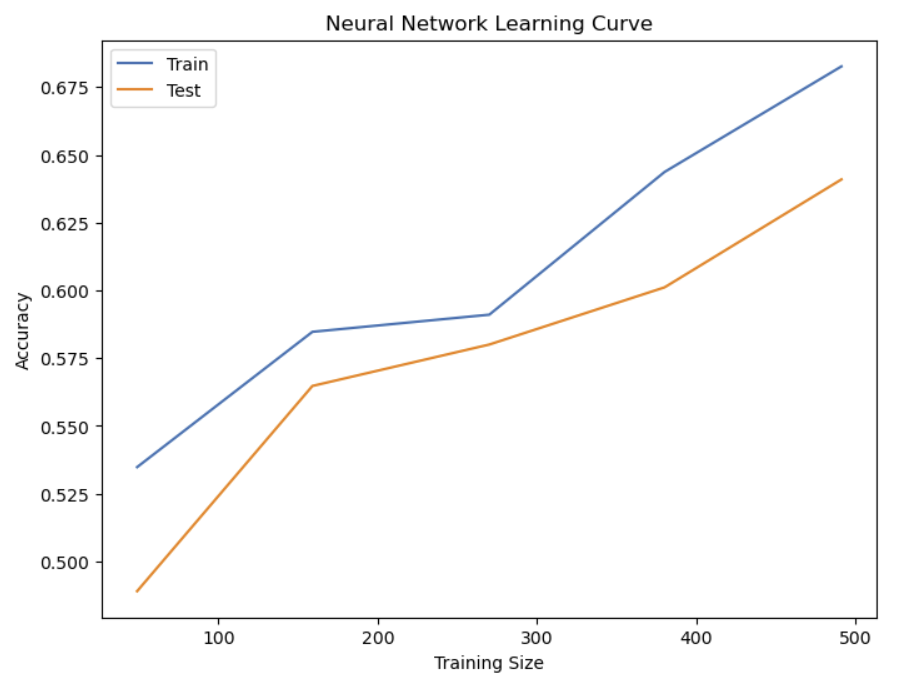
\includegraphics[width=0.40\textwidth]{PIMA Indian Diabetes Graphs/Neural Nets/nn init lc.png}
    \label{fig:enter-label}
\end{figure}

\begin{figure}[H]
    \centering
    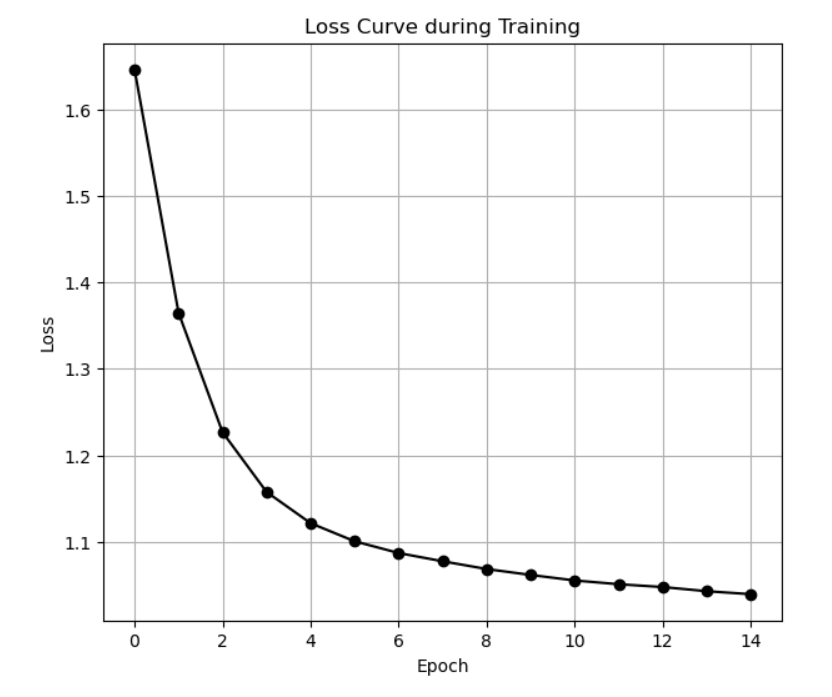
\includegraphics[width=0.40\textwidth]{PIMA Indian Diabetes Graphs/Neural Nets/nn loss curve.png}
    \label{fig:enter-label}
    \caption{Loss drops off extensively by 14 epochs}
\end{figure}

This learning curve is really interesting. What I took away from this one is that both the training and testing datasets perform much better when they are allowed to see more data. If I had access to more data, maybe these would converge closer to each other. But this graph gives the impression that there is not much bias or variance in the data, which is a different illustration than the decision tree, for example. After performing hyperparameterization with GridSearchCV, I received input that the best combination of parameters was as follows: {activation=tanh}, {early\_stopping=True}, {hidden\_layer\_sizes=(128, 64, 32)}, {max\_iter=1000}, {random\_state=42}. See learning curve below:

\begin{figure}[H]
    \centering
    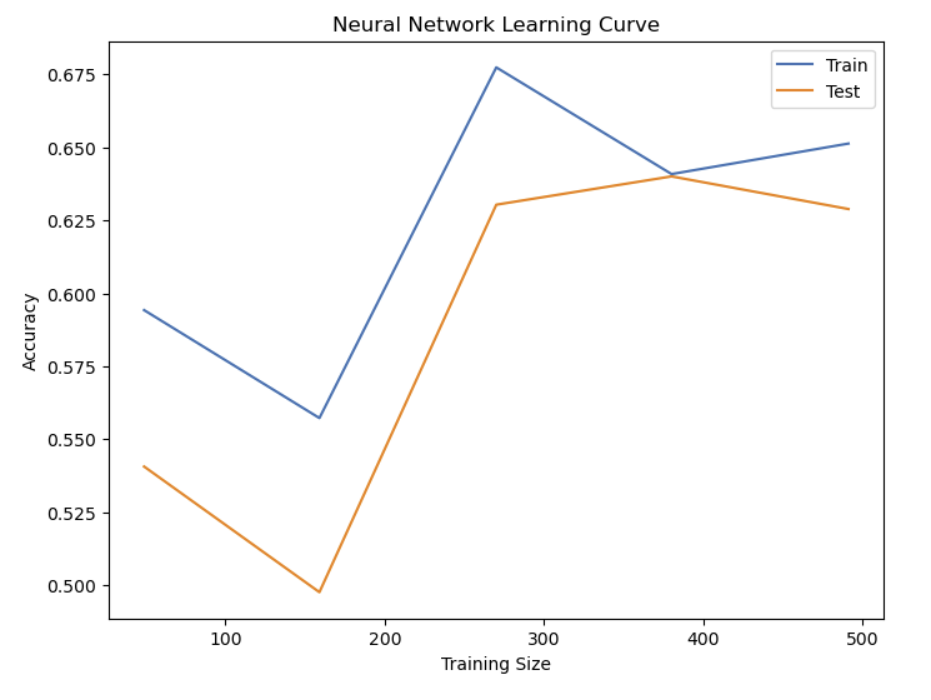
\includegraphics[width=0.40\textwidth]{PIMA Indian Diabetes Graphs/Neural Nets/nn fin lc.png}
    \label{fig:enter-label}
\end{figure}

The final MLP has a better ability to learn. Another thing of contention that this curve demonstrates high variance on the left, but it converges to an f1\_weighted of around 0.651. 

One thing that both the initial and final learning curve seem to agree on was the idea that more hidden layers actually hurts the f1\_weighted score, and the graph below illustrates this:

\begin{figure}[H]
    \centering
    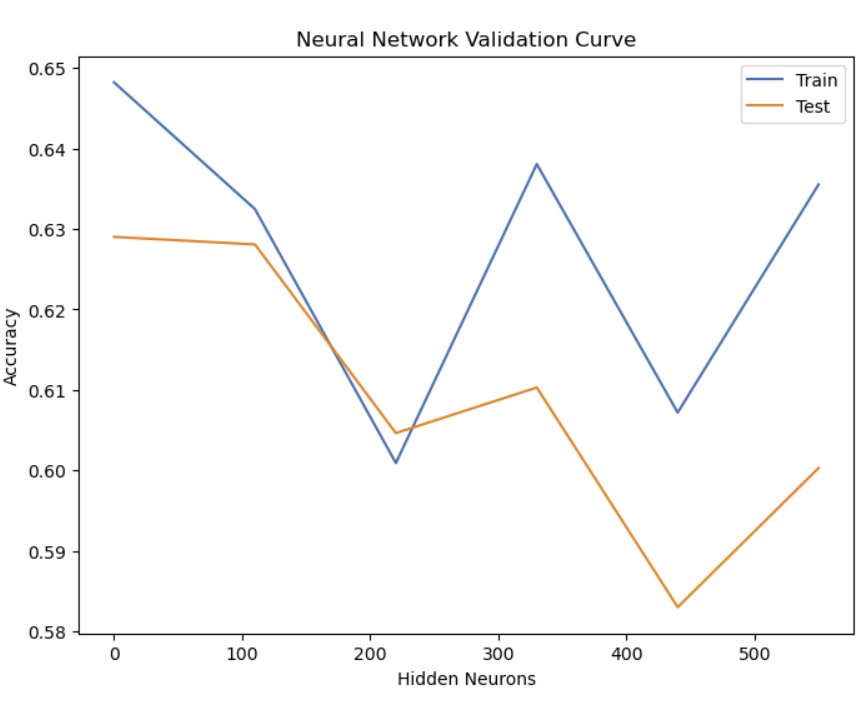
\includegraphics[width=0.40\textwidth]{PIMA Indian Diabetes Graphs/Neural Nets/nn val.png}
    \label{fig:enter-label}
\end{figure}

At the end of hyperparameterization, the MLP was able to ascertain an f1\_weighted score of 0.65161. Compared to the decision tree example, this algorithm did not see as drastic of an improvement. I hypothesize this is because of the inherent nature of the algorithm. It can try more combinations of inputs, but is limited by the fact that there was not much data to go off of, whereas decision trees can do well without large amounts of data. The classification below report demonstrates the strong ability of the MLP to perform. Both the precision and recall scores were around 70-75 percent accurate.

\begin{figure}[H]
    \centering
    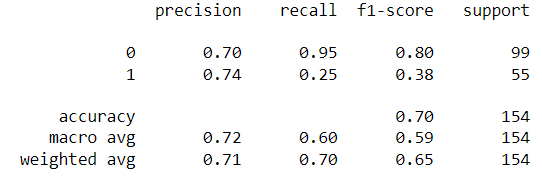
\includegraphics[width=0.40\textwidth]{PIMA Indian Diabetes Graphs/Neural Nets/nn cr.png}
    \label{fig:enter-label}
\end{figure}

Wall Clock Time: 
\begin{figure}[H]
    \centering
    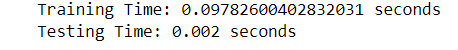
\includegraphics[width=0.40\textwidth]{PIMA Indian Diabetes Graphs/Neural Nets/nn wct.png}
    \label{fig:enter-label}
    \caption{the test data fit very quickly}
\end{figure}

\subsection{\textbf{Red Wine Quality Dataset}}\label{BB}
For my baseline MLP, I initialized it with the following parameters: {max\_iter=1000}, {early\_stopping=True}, {validation\_fraction=0.1}, {n\_iter\_no\_change=10},  {random\_state=42}, and {learning\_rate\_init=0.001}. From this, my initial f1\_weighted score was 0.47786.

\begin{figure}[H]
    \centering
    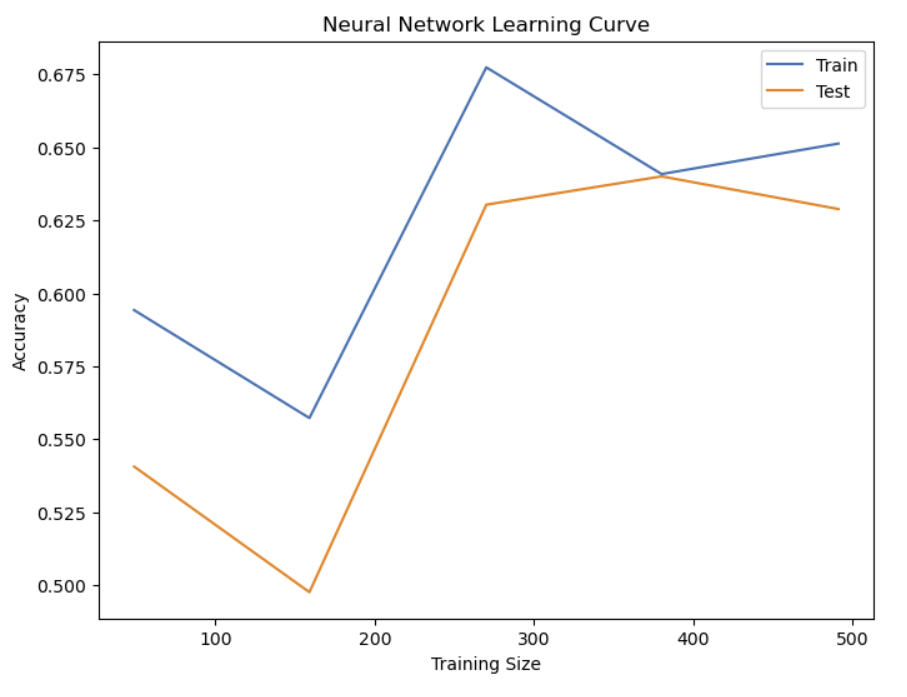
\includegraphics[width=0.40\textwidth]{Red Wine Quality Graph Images/Neural Nets/nn lc init.png}
    \label{fig:enter-label}
    \caption{Unlike most of my initial learning curves, these actually converge around 400 records for training size}
\end{figure}

\begin{figure}[H]
    \centering
    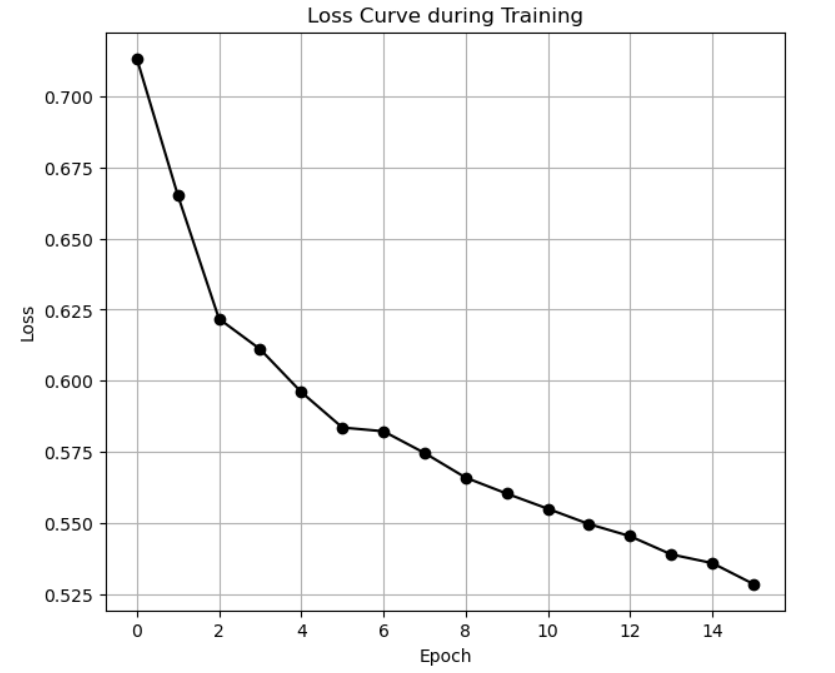
\includegraphics[width=0.40\textwidth]{Red Wine Quality Graph Images/Neural Nets/nn loss curve.png}
    \label{fig:enter-label}
    \caption{Loss drops off extensively by 15 epochs}
\end{figure}

This learning curve is really interesting. Both the training and testing splits perform best around 400 records. After performing hyperparameterization with GridSearchCV, I received input that the best combination of parameters was as follows: {activation='tanh'}, {alpha=0.001}, {early\_stopping=True},{hidden\_layer\_sizes=(64, 32)}, {max\_iter=1000}, {random\_state=42}. See learning curve below:

\begin{figure}[H]
    \centering
    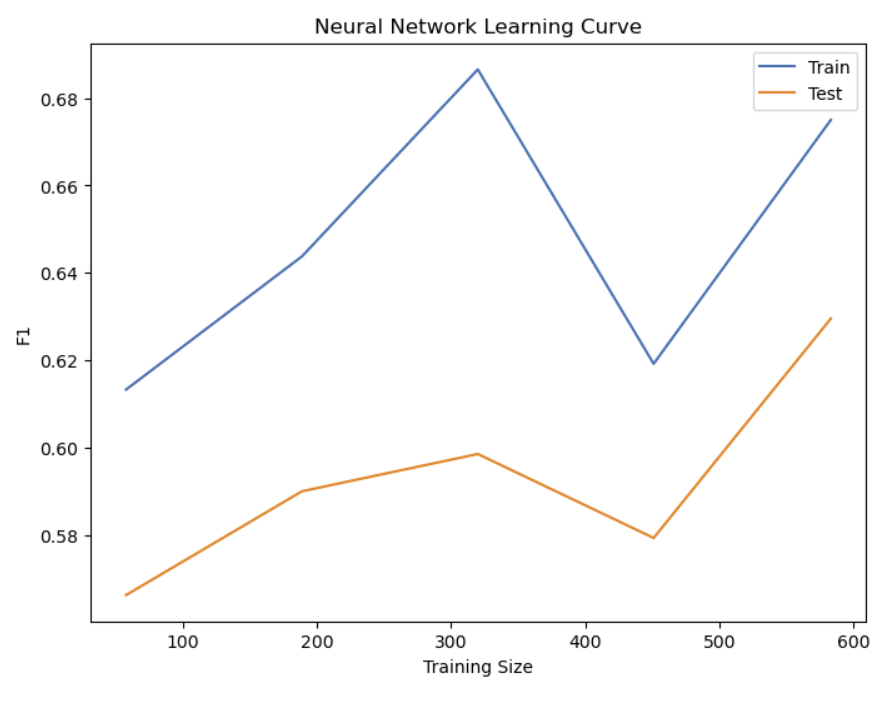
\includegraphics[width=0.40\textwidth]{Red Wine Quality Graph Images/Neural Nets/nn lc final.png}
    \label{fig:enter-label}
\end{figure}

The final MLP performed worse. Another thing of contention that this curve demonstrates high variance on the left, but it converges to an f1\_weighted of around 0.45203. 

One thing that both the initial and final learning curve seem to agree on was the idea that more hidden layers actually hurts the f1\_weighted score, and the graph below illustrates this:

\begin{figure}[H]
    \centering
    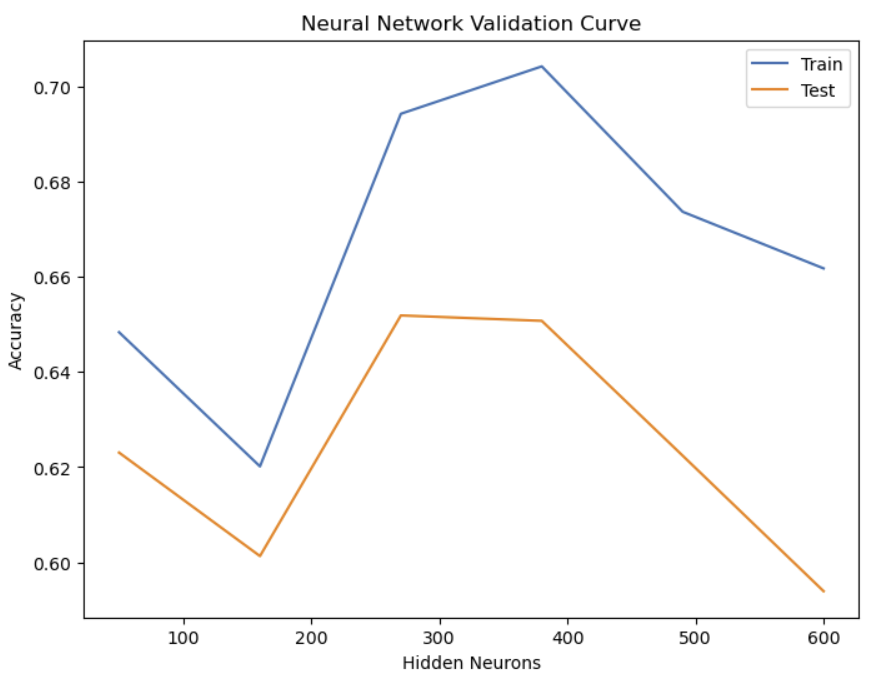
\includegraphics[width=0.40\textwidth]{Red Wine Quality Graph Images/Neural Nets/nn vc final.png}
    \label{fig:enter-label}
\end{figure}

At the end of hyperparameterization, the MLP was able to ascertain an f1\_weighted score of 0.45203. Compared to the decision tree example, this algorithm did not see as drastic of an improvement. Similar to the PIMA Indians Diabetes dataset, I hypothesize this is because of the inherent nature of the algorithm. Again, it attempts many combinations of inputs, but is limited by the fact that there was not much data to go off of. The classification below report demonstrates the weak ability of the MLP to perform. For wine quality values of 3, 4, and 8, it received a precision and recall score of 0.

\begin{figure}[H]
    \centering
    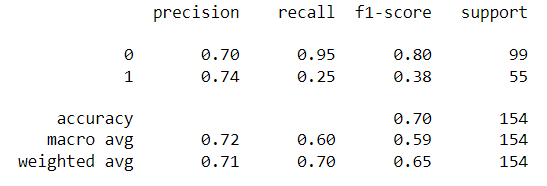
\includegraphics[width=0.40\textwidth]{Red Wine Quality Graph Images/Neural Nets/nn cr.png}
    \label{fig:enter-label}
\end{figure}

Wall Clock Time: 
\begin{figure}[H]
    \centering
    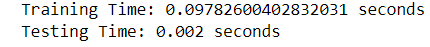
\includegraphics[width=0.40\textwidth]{Red Wine Quality Graph Images/Neural Nets/nn wct.png}
    \label{fig:enter-label}
    \caption{the test data fit almost instantaneously}
\end{figure}

This algorithm, along with SVMs, takes a very long time to run. When contrasting this with KNN or Decision Trees, it also felt like it required my processing power. All other processes on my machine seemed to halt when trying to execute this algorithm.

\section{SVM}

\subsection{\textbf{PIMA Indians Diabetes Dataset}}\label{AA}
This section was the most interesting of them all, in my opinion. Because of the complexity of data, I wanted to try my hand at the C value (regularization parameter) to see its effects on the f1\_weighted score. This algorithm took a \emph{ages} compared to the other data set to train my initial models. Although the beginning f1\_weighted score was 0.75324, considerably higher than other algorithms, it took a whopping 14 seconds to train the data. Once it was trained, though, the testing time was about 0.00327 seconds. 

\begin{figure}[H]
    \centering
    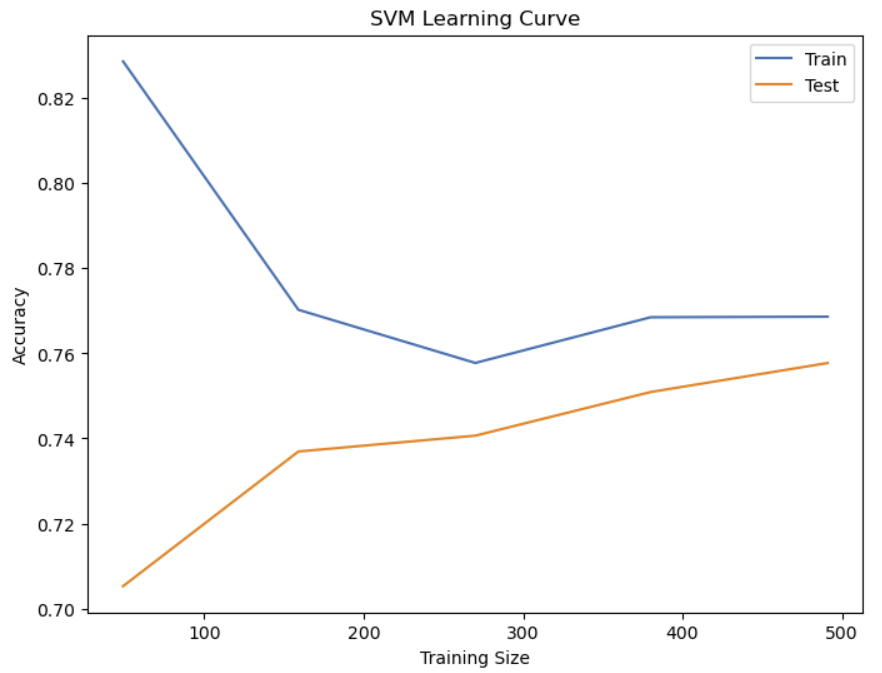
\includegraphics[width=0.40\textwidth]{PIMA Indian Diabetes Graphs/SVC/svc init lc.png}
    \label{fig:enter-label}
\end{figure}

GridSearchCV came back with the following values: C=0.1, kernel=linear,probability=True, random\_state=42. From this, I can deduce that the algorithm is preferring to use a larger margin. Additionally, the data are linearly separable, because I asked GridSearchCV to try other kernels like poly and rbf, but this was still the best option available. Updated learning and validation curve:

\begin{figure}[H]
    \centering
    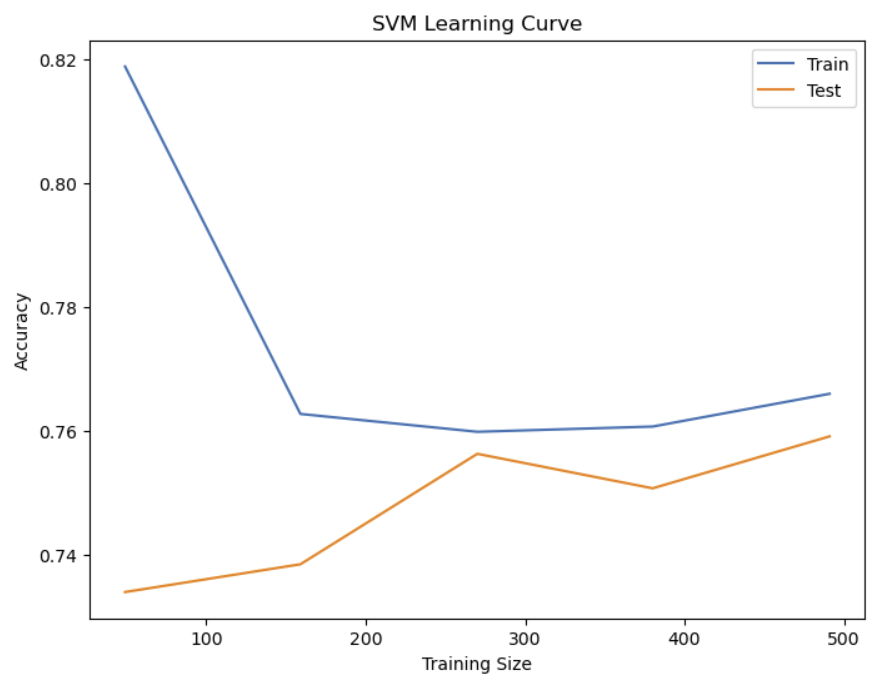
\includegraphics[width=0.40\textwidth]{PIMA Indian Diabetes Graphs/SVC/svc fin lc.png}
    \label{fig:enter-label}
    \caption{High variance, but little bias, suggesting overfit}
\end{figure}

\begin{figure}[H]
    \centering
    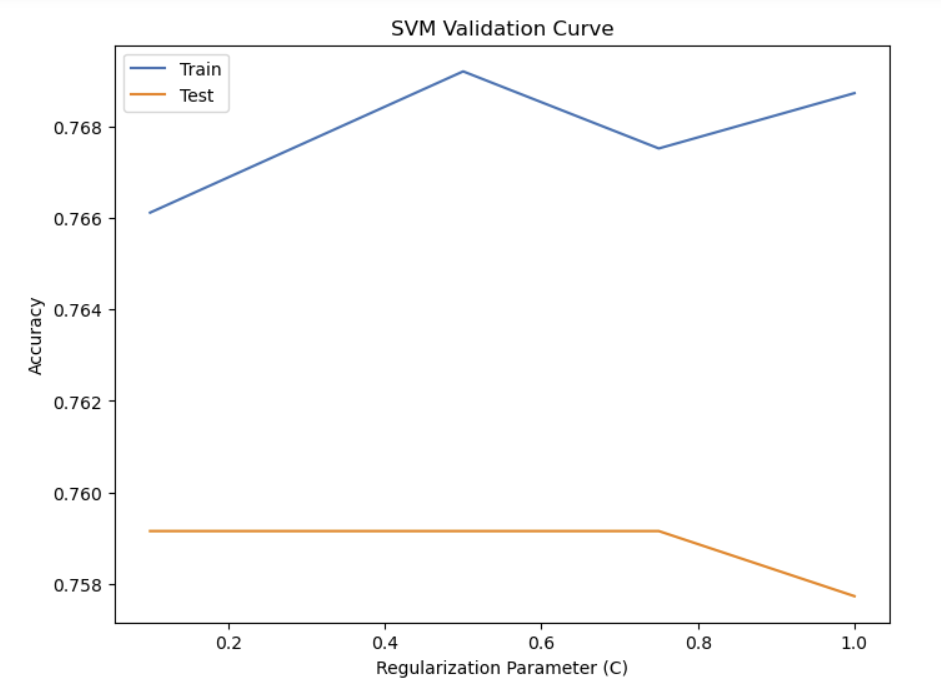
\includegraphics[width=0.40\textwidth]{PIMA Indian Diabetes Graphs/SVC/svc vc.png}
    \label{fig:enter-label}
\end{figure}

For the second learning curve, we see some improvement, although the high variance remains the same. However, the part that makes this analysis interesting is the validation curve. The training set has a much higher f1\_weighted score, and for the test curve, it does not benefit whatsoever from larger C values. In fact, at C=1, it actually hurts the score. This indicates that the data are prefer having a larger margin, meaning that there are not labels that are close to each other. If the algorithm could operate on a higher C value, it would. Although GridSearchCV recommended the linear kernel, the learning and validation curves from the RBF kernel did reasonably well. 

\begin{figure}[H]
    \centering
    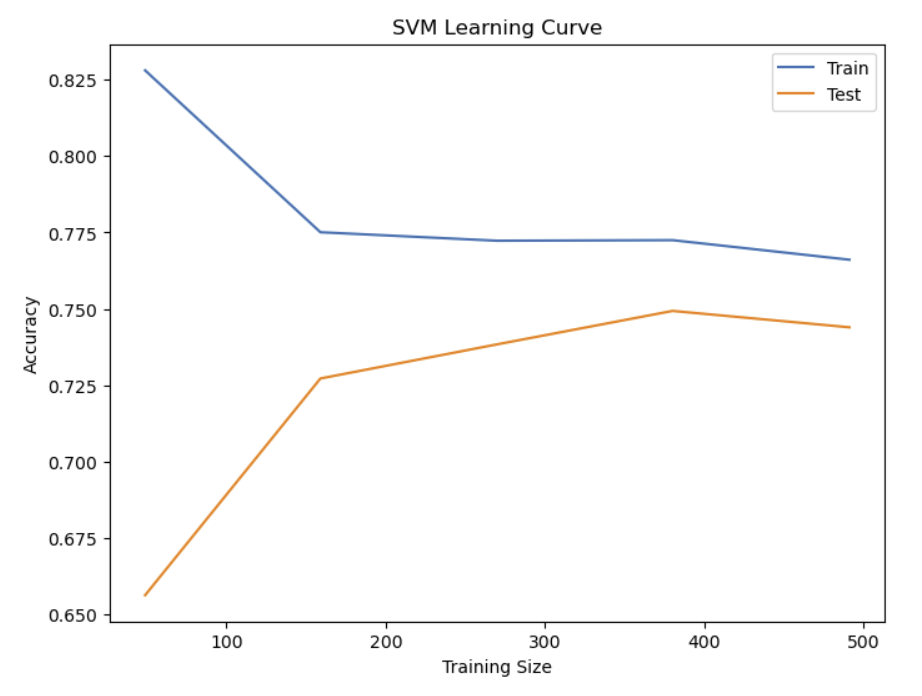
\includegraphics[width=0.40\textwidth]{PIMA Indian Diabetes Graphs/SVC/svc rbf lc.png}
    \label{fig:enter-label}
    \caption{High variance in the RBF kernel, but similar bias to the linear kernel}
\end{figure}

\begin{figure}[H]
    \centering
    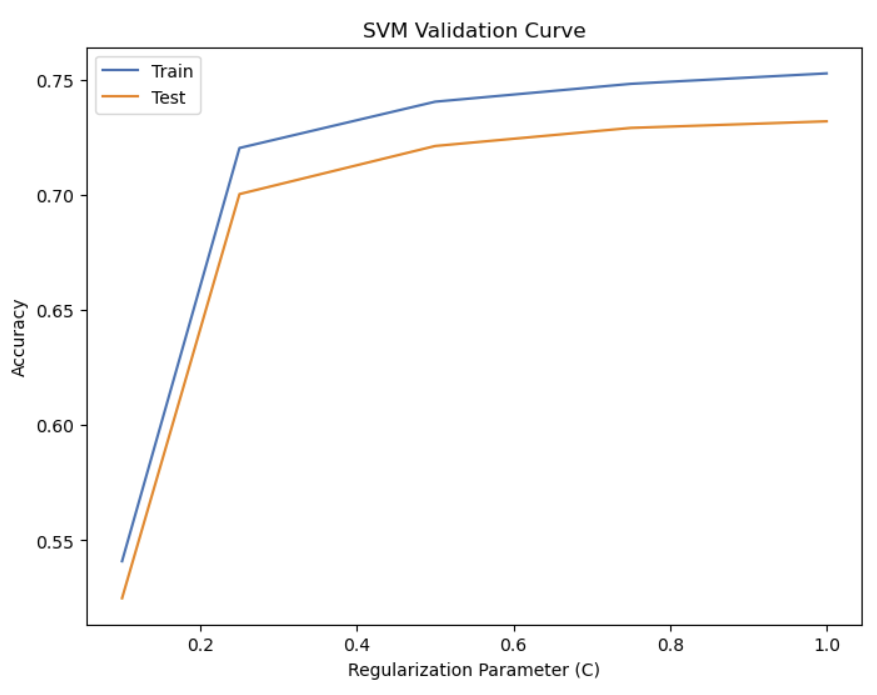
\includegraphics[width=0.40\textwidth]{PIMA Indian Diabetes Graphs/SVC/svc rbf vc.png}
    \label{fig:enter-label}
\end{figure}

This algorithm produced an F1\_weighted score of 0.7586. The interesting part about using the RBF kernel was the wall clock time. It initialized noticeably quicker than the linear kernel. Because they both performed similarly, it suggests that the data are most likely linearly-separable. However, the F1\_weighted score did perform similarly in the training and test sets.

In terms of classification, the SVM with a linear kernel does a relatively good job here as well: 

\begin{figure}[H]
    \centering
    \includegraphics[width=0.40\textwidth]{PIMA Indian Diabetes Graphs/SVC/svc cr.png}
    \label{fig:enter-label}
\end{figure}

The weighted avg for the f1 score is in the same ballpark as all the other algorithms for detecting no diabetes, but not as high for detecting when someone does in fact have diabetes. It only get this correct about two-thirds of the time.

Additionally, this algorithm fits data extremely slow when compared to the other algorithms. The data were even scaled using a MinMaxScaler. This had little-to-no effect on the data. This tells me that SVMs are inherently slow, even with small amounts of data.

\begin{figure}[H]
    \centering
    \includegraphics[width=0.40\textwidth]{PIMA Indian Diabetes Graphs/SVC/svc wct.png}
    \label{fig:enter-label}
\end{figure}

\subsection{\textbf{Red Wine Quality Dataset}}\label{BB}

For this dataset, I experimented with the linear and rbf kernels as well. The linear kernel, with a C=1 performed better than the rbf kernel with the same C value. The initial learning curve for the linear kernel got an F1\_weighted score of 0.75324, whereas the rbf kernel received an F1\_weighted score of 0.7586. Although the rbf kernel did better initially, the GridSearchCV determined that the linear kernel was better overall. 

\begin{figure}[H]
    \centering
    \includegraphics[width=0.40\textwidth]{Red Wine Quality Graph Images/SVC/svm lin lc init.png}
    \label{fig:enter-label}
    \caption{SVM Linear Kernel Initial Learning Curve}
\end{figure}
High bias, high variance with this initial linear kernel model. 

\begin{figure}[H]
    \centering
    \includegraphics[width=0.40\textwidth]{Red Wine Quality Graph Images/SVC/svm rbf lc.png}
    \label{fig:enter-label}
    \caption{SVM RBF Kernel Learning Curve}
\end{figure}
The kernel change here to RBF did not make a significant difference.

\begin{figure}[H]
    \centering
    \includegraphics[width=0.40\textwidth]{Red Wine Quality Graph Images/SVC/svm lin vc init.png}
    \label{fig:enter-label}
    \caption{SVM Linear Kernel Initial Validation Curve}
\end{figure}

\begin{figure}[H]
    \centering
    \includegraphics[width=0.40\textwidth]{Red Wine Quality Graph Images/SVC/svm rbf vc.png}
    \label{fig:enter-label}
    \caption{SVM RBF Kernel Validation Curve}
\end{figure}
The validation curves also do not look very different: low variance and high bias, which is likely due to this model's inability to fit correctly (underfit). 

The GridSearchCV hyperparameterization gave the following parameters: C=0.1, kernel='linear', probability=True, random\_state=42. Given this fact, it is evident that the data are more suited to be linearly separable. With this, the learning curve and validation curve looked like the following:

\begin{figure}[H]
    \centering
    \includegraphics[width=0.40\textwidth]{Red Wine Quality Graph Images/SVC/svm lin lc fin.png}
    \label{fig:enter-label}
    \caption{SVM Linear Kernel Final Validation Curve}
\end{figure}

\begin{figure}[H]
    \centering
    \includegraphics[width=0.40\textwidth]{Red Wine Quality Graph Images/SVC/svm lin vc fin.png}
    \label{fig:enter-label}
    \caption{SVM Linear Kernel Final Validation Curve}
\end{figure}

The learning curve, although starting with a high variance, ends up having less bias at the end. The two curves do not converge to a specific value, but they come much closer together than the earlier two learning curves. The interesting portion from this was the validation curve. It objectively performs better for both the training and testing splits (the f1\_weighted score is higher for both, but when C is approximately 0.75, the training and testing validation curves perform opposite of each other. One possible explanation for this is that the training data are more sparsely-plotted when compared to the test data. Because a higher C value reduces the strength of regularization, it allows the SVM to fit the training data more closely, thereby increasing the f1\_weighted score. 

\begin{figure}[H]
    \centering
    \includegraphics[width=0.40\textwidth]{Red Wine Quality Graph Images/SVC/svm cr.png}
    \label{fig:enter-label}
    \caption{SVM Classification Report - Not able to perform well on the higher and lower bounds of quality}
\end{figure}

\begin{figure}[H]
    \centering
    \includegraphics[width=0.40\textwidth]{Red Wine Quality Graph Images/SVC/svm wct.png}
    \label{fig:enter-label}
    \caption{SVM Wall Clock Time}
\end{figure}

\section{Conclusions, Final Takeaways}
The overall accuracy of each model was very similar, for both datasets: for the PIMA Indians Diabetes dataset, the accuracy hovered around 50 percent, and for the Red Wine Quality dataset, it hovered around 75 percent. The same could be said the f1\_weighted score as well: for the first dataset (PIMA), it hovered around 0.50 again, and for the second dataset (RWQ), it hovered around 0.75 again, ironically. For ease of use, see the tables below for each dataset and their respective accuracies and f1-weighted scores.

\bibliographystyle{plain}
\bibliography{references}
\cite{cortez2009red}
\cite{smith1988pima}

\end{document}
